\documentclass[aspectratio=169,xcolor=dvipsnames]{beamer}
\usetheme{SimpleDarkBlue}
\usepackage{multirow}
\usepackage{booktabs}
\usepackage{hyperref}
\usepackage{graphicx}
\usepackage{booktabs} 
\usepackage{amssymb}
\usepackage{amsmath}
\usepackage{tikz}
\usepackage{xcolor}
\usepackage{caption}
\usepackage{amsthm}
\usepackage{fontawesome5}

\title{Modern Methods in Video Anomaly Detection: A Review}

\author{
	Mohammad Hosein Rabiee
}

\institute
{
	Department of Computer Science and Statistics \\
	Faculty of Mathematics \\
	K. N. Toosi University of Technology
}
\date{}

\begin{document}
	
	\begin{frame}
		\titlepage
	\end{frame}
	
	\begin{frame}{{Introduction to Video Anomaly Detection}}
		\small
		\begin{itemize}
			\item \textbf{Video Anomaly Detection (VAD)} focuses on identifying 
			events that deviate from normal patterns in surveillance, traffic, and 
			safety-critical environments.
			
			\item VAD is challenging because anomalies are 
			\textcolor{red}{rare}, \textcolor{red}{diverse}, and often 
			\textcolor{red}{ill-defined}, requiring reliable and interpretable systems.
			
			\item \textbf{Existing deep learning–based VAD approaches} include 
			supervised, weakly supervised, and unsupervised paradigms.  
			\begin{itemize}
				\item These methods often struggle with \textcolor{red}{performance} and \textcolor{red}{requirement of substantial data}.
			\end{itemize}
			
			\item The rise of \textbf{Multimodal Large Language Models (MLLMs)} 
			introduces new opportunities for VAD because of their ability to 
			\textcolor{cyan}{jointly process and reason over visual and textual information},  
			opening promising new research directions.
			
		\end{itemize}
	\end{frame}
	
	\begin{frame}{Papers for Review}
		\small
		\begin{itemize}
			\item \faFile \hspace{0.3cm} 
			{\color{cyan}\textbf{VERA: Explainable Video Anomaly Detection}} {\color{gray}(2024)}
			
			\vspace{0.3cm}
			\item \faFile\hspace{0.3cm} 
			{\color{cyan}\textbf{HiProbe-VAD: A Tuning-Free MLLM-Based Framework for Video Anomaly Detection}} {\color{gray}(2025)}
			
			\vspace{0.3cm}
			\item \faFile\hspace{0.3cm} 
			{\color{cyan}\textbf{EventVAD: Event-based Video Anomaly Detection}} {\color{gray}(2024)}
		\end{itemize}
	\end{frame}
	
	\begin{frame}{VERA: Core Idea}
		\small
		
		\begin{block}{Key Observation}
			Despite the promise of MLLMs, existing VLM-based VAD approaches face two main limitations:
			\begin{itemize}
				\item use of \textbf{\textcolor{cyan}{external LLM reasoning modules}} 
				→ high inference cost,
				\item reliance on \textbf{\textcolor{cyan}{instruction tuning}} 
				→ requires expensive frame-level annotations.
			\end{itemize}
			We need	a method that keeps VLMs frozen while still enabling 
			strong reasoning and interpretability.
		\end{block}
		
		\begin{alertblock}{Proposed Framework: VERA}
			\textbf{VERA} is introduced to overcome these challenges by enabling  
			effective reasoning \textbf{without modifying or tuning the VLM itself}.
			
		\end{alertblock}
		\begin{block}{Key insight}
			VERA learns a collection of \textbf{\textcolor{red}{guiding questions}} that act as \textbf{trainable parameters}..
		\end{block}
	\end{frame}
	
	
	\begin{frame}{VERA: Core Idea (Cont.)}
		
		\begin{figure}
			\centering
			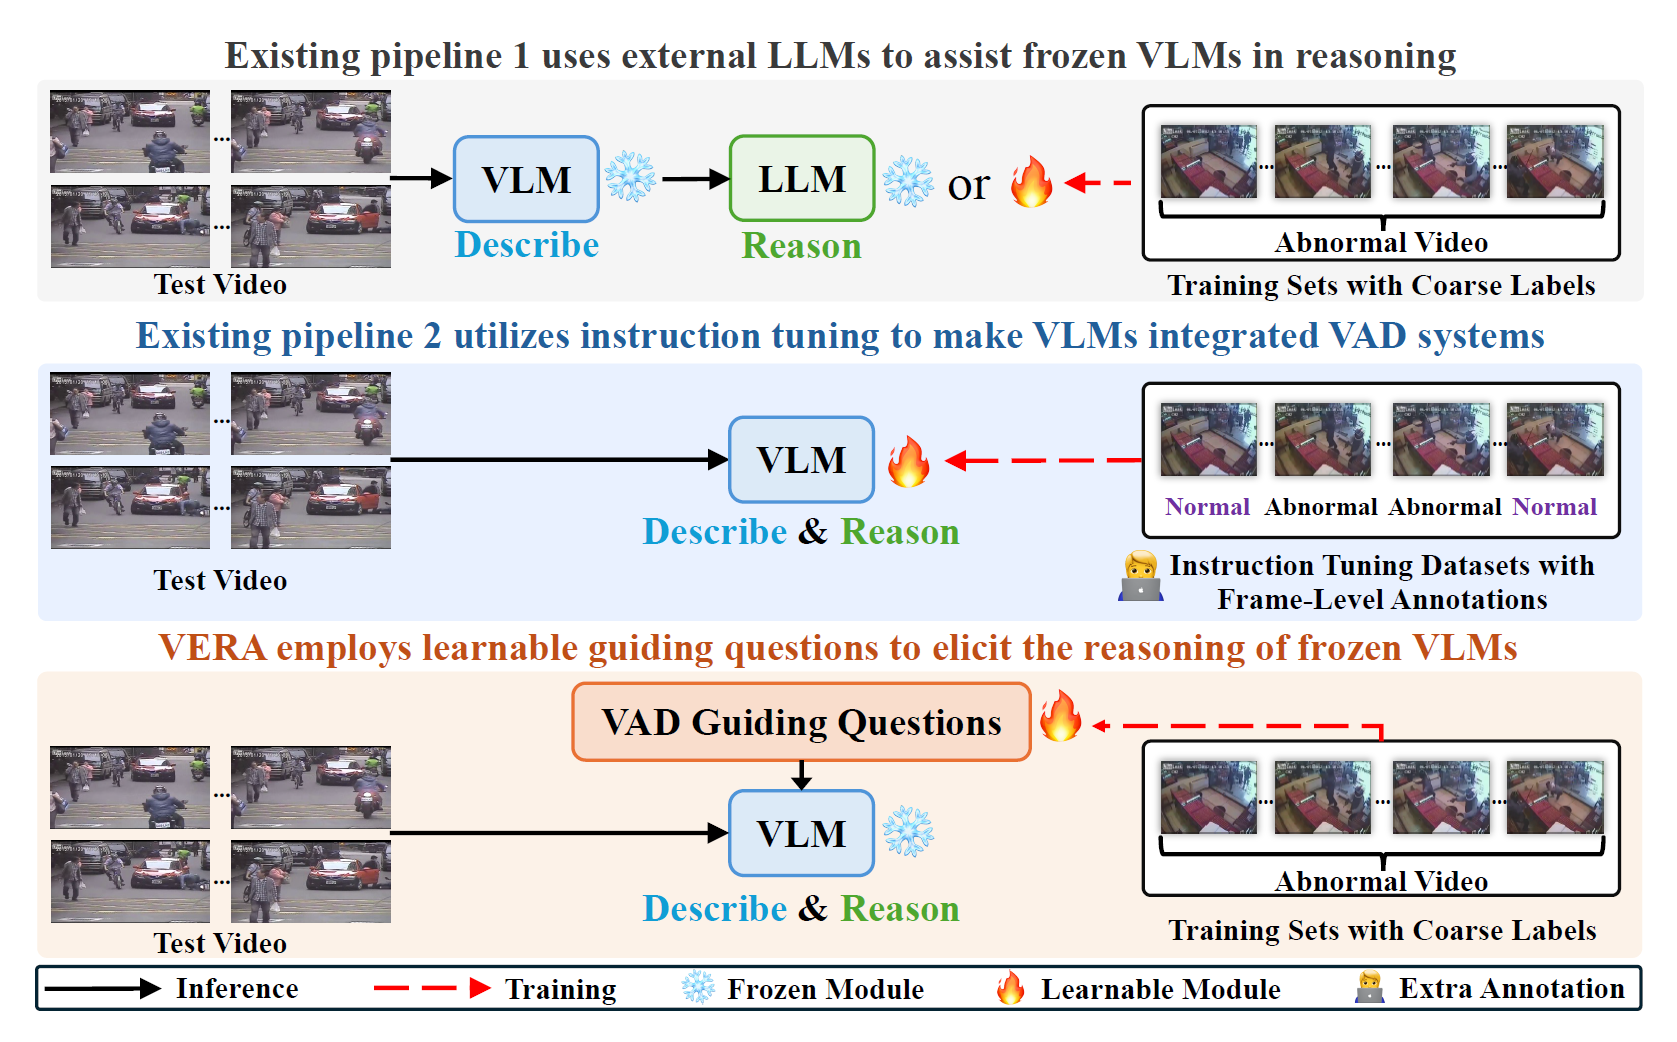
\includegraphics[width=0.7\linewidth]{images/VERA_Figure1.png}
			\caption{VERA renders frozen VLMs to describe and reason with learnable
				guiding questions learned from coarsely labeled data.}
		\end{figure}
		
		\vspace{0.5em}
		
		
	\end{frame}
	
	
	\begin{frame}{VAD: Problem Formulation}
		\small
		
		\begin{block}{Video Anomaly Detection Setting}
			Let \(V = \{I_i\}_{i=1}^{F}\) be a video containing \(F\) frames, where \(I_i\) is the \(i\)-th frame.
			The goal of VAD is to detect the start and end of anomalous events within the video.
		\end{block}
		
		\begin{block}{Frame-Level Labels}
			\begin{itemize}
				\item Each frame is assigned a binary label:
				\[
				y_i \in \{0,1\}
				\]
				\item \(y_i = 1\) indicates an anomalous frame
				\item \(y_i = 0\) indicates a normal frame
			\end{itemize}
		\end{block}
		
		\begin{block}{VERA Objective}
			VERA uses a frozen VLM \(f_{\mathrm{VLM}}\) to predict continuous anomaly scores:
			\[
			\hat{Y} = [\hat{y}_1, \dots, \hat{y}_F], \qquad \hat{y}_i \in [0,1]
			\]
		\end{block}
		
	\end{frame}
	
	\begin{frame}{VAD: Training Data}
		\small
		
		\begin{block}{Coarsely Labeled Training Sets}
			VAD datasets typically provide only \textbf{\textcolor{red}{video-level labels}} rather than frame-level annotations.
		\end{block}
		
		\begin{itemize}
			\item Training set:
			\[
			D = \{(V^{(j)}, Y^{(j)})\}_{j=1}^{N}
			\]
			where \(N\) is the number of training videos.
			
			\item For each video \(V^{(j)}\):
			\[
			V^{(j)} = \{ I^{(j)}_i \}_{i=1}^{F_j}
			\]
			
			\item Label meaning:
			\begin{itemize}
				\item \(Y^{(j)} = 1\) → video contains \textcolor{red}{at least one anomaly}
				\item \(Y^{(j)} = 0\) → video contains \textcolor{red}{no anomalies}
			\end{itemize}
			
			\item No fine-grained annotations such as frame-level \(y_i\).
			
		\end{itemize}
		
		
	\end{frame}
	
	\begin{frame}{Training Objective}
		\small
		
		\begin{block}{Goal}
			We aim to learn guiding questions that break down the complex and ambiguous concept of 
			\textbf{\textcolor{red}{“anomaly”}}  
			into identifiable anomalous patterns.  
			These patterns vary across datasets, making manually designed descriptions ineffective for generalization.
		\end{block}
		
		\begin{itemize}
			\item VERA proposes a general VL framework to automatically generate such guiding questions.
			\item Guiding question set:
			\[
			Q = \{ q_1, \ldots, q_m \}, \quad q_i \text{ is the } i\text{-th question},\; 1 \le i \le m
			\]
			\item The set \(Q\) is treated as \textbf{\textcolor{red}{learnable parameters}}.
			\item Optimization occurs through \textbf{verbal interaction} between:
			\begin{itemize}
				\item a learner  
				\item an optimizer  
			\end{itemize}
			both modeled by VLMs via instruction-following prompts.
		\end{itemize}
		
	\end{frame}
	
	
	\begin{frame}{Training Data}
		
		\begin{block}{Training Data}
			Paired sampled frames and video-level labels are used. Sampling is required due to the large number of frames.
		\end{block}
		
		\begin{itemize}
			\item Uniform sampling yields the best performance.
			\item For any video \(V^{(j)} \in D\):
			\[
			\ell = \left\lfloor \frac{F_j}{S} \right\rfloor
			\]
			where \(S\) is the number of sampled frames.
			\item Sampled frame sequence:
			\[
			\tilde{V}^{(j)} = 
			\big[\, I^{(j)}_{1},\, I^{(j)}_{\ell+1},\, \ldots,\, I^{(j)}_{(S-1)\ell + 1} \,\big]
			\]
			\item Training pairs:
			\[
			\{\, (\tilde{V}^{(j)},\, Y^{(j)}) \,\}_{j=1}^{N}
			\]
		\end{itemize}
		
	\end{frame}
	
	
	
	\begin{frame}{Updating \(Q\) via Learner and Optimizer}
		\small
		
		\begin{block}{Verbalized Optimization (VML)}
			Since guiding questions \(Q\) are \textbf{\textcolor{red}{verbal expressions of anomaly patterns}},
			VERA optimizes them via verbal communication between:
			
			\[
			f_{\text{learner}} \quad \text{and} \quad f_{\text{opt}}
			\]
			
			instead of numerical optimizers (e.g., Adam).
		\end{block}
		
		\begin{block}{General VL Formulation}
			Any LLM-based model is written as:
			\[
			f(x; \phi)
			\]
			where:
			\begin{itemize}
				\item \(x\): input data
				\item \(\phi\): natural-language instructions (treated as learnable parameters)
			\end{itemize}
		\end{block}
		
		
	\end{frame}
	
	\begin{frame}{Learner at Iteration \(t\)}
		\small
		
		\begin{block}{Learner Agent}
			The learner is modeled by the frozen VLM \(f_{\text{VLM}}\)
			with prompt template \(\theta\):
			
			\[
			f^{(t)}_{\text{learner}}(x)
			=
			f_{\text{VLM}}(x; (\theta, Q_t))
			\]
			
			\begin{itemize}
				\item \(x\): input for the learning task
				\item \((\theta, Q_t)\): task prompt + current guiding questions
				\item \(Q_t\): guiding questions at iteration $t$
			\end{itemize}
		\end{block}
	\end{frame}
	
	\begin{frame}{Optimizer at Iteration \(t\)}
		\small
		\begin{block}{Optimizer Agent}
			The optimizer evaluates predictions and refines \(Q_t\):
			
			\[
			f^{(t)}_{\text{opt}}(z)
			=
			f_{\text{VLM}}(z; (\psi, Q_t))
			\]
			
			\begin{itemize}
				\item \(z\): optimizer input
				\item \(\psi\): instruction to improve \(Q_t\)
				\item \textbf{\(f^{(t)}_{\text{learner}} \neq f^{(t)}_{\text{opt}}\)}
			\end{itemize}
			
		\end{block}
		
		
	\end{frame}
	
	\begin{frame}{Learning Task for \(f_{\text{learner}}\)}
		\small
		
		\begin{block}{Forward Pass of the Learner}
			The learner performs the forward pass and outputs a prediction
			using only the \textbf{\textcolor{red}{coarsely labeled training data}}.
		\end{block}
		
		\begin{itemize}
			\item A \textbf{binary classification task} is designed for the learner.
			\item It considers:
			\begin{itemize}
				\item temporal nature of video data
				\item sparsity of anomalies
				\item weak supervision in VAD datasets
			\end{itemize}
		\end{itemize}
		
		
		\begin{itemize}
			\item The task description is written in the \textbf{Model Description} section of the prompt template \(\theta\).
			\item The guiding questions \(Q_t\) are inserted into the \textbf{Prompt Questions} section to trigger reasoning in the VLM.
		\end{itemize}
		
	\end{frame}
	
	
	\begin{frame}{Optimization Step in \(f_{\text{opt}}\)}
		\small
		
		\begin{block}{Backward Pass of the Optimizer}
			The optimizer performs the \textbf{\textcolor{red}{backward pass}} to update the guiding
			questions \(Q_t\) using a mini-batch of size \(n\).
		\end{block}
		
		\begin{itemize}
			\item Let the batched visual inputs be:
			\[
			V_{\text{batch}}
			=
			[\tilde{V}^{(1)}_{\text{batch}}, \ldots, \tilde{V}^{(n)}_{\text{batch}}]
			\]
			\item The corresponding ground-truth video-level labels:
			\[
			Y_{\text{batch}}
			=
			[Y^{(1)}_{\text{batch}}, \ldots, Y^{(n)}_{\text{batch}}]
			\]
		\end{itemize}
		
		
		
	\end{frame}
	
	\begin{frame}{Optimization Step in \(f_{\text{opt}}\) (Cont.)
		}
		\small
		\begin{block}{Learner Predictions}
			Using current \(Q_t\), the learner produces:
			\[
			\hat{Y}_{\text{batch}}
			=
			[\hat{Y}^{(1)}_{\text{batch}}, \ldots, \hat{Y}^{(n)}_{\text{batch}}]
			\]
		\end{block}
		
		\begin{block}{Optimizer Update Rule}
			After reading the batched data and predictions, the optimizer generates a new question set:
			\[
			Q_{t+1}
			=
			f^{(t)}_{\text{opt}}(V_{\text{batch}},\, \hat{Y}_{\text{batch}},\, Y_{\text{batch}})
			\]
			where \(Q_{t+1}\) is produced through the text-generation and
			instruction-following abilities of the frozen VLM.
		\end{block}
		
	\end{frame}
	
	\begin{frame}{Overall Training Pipeline}
		
		\begin{figure}
			\centering
			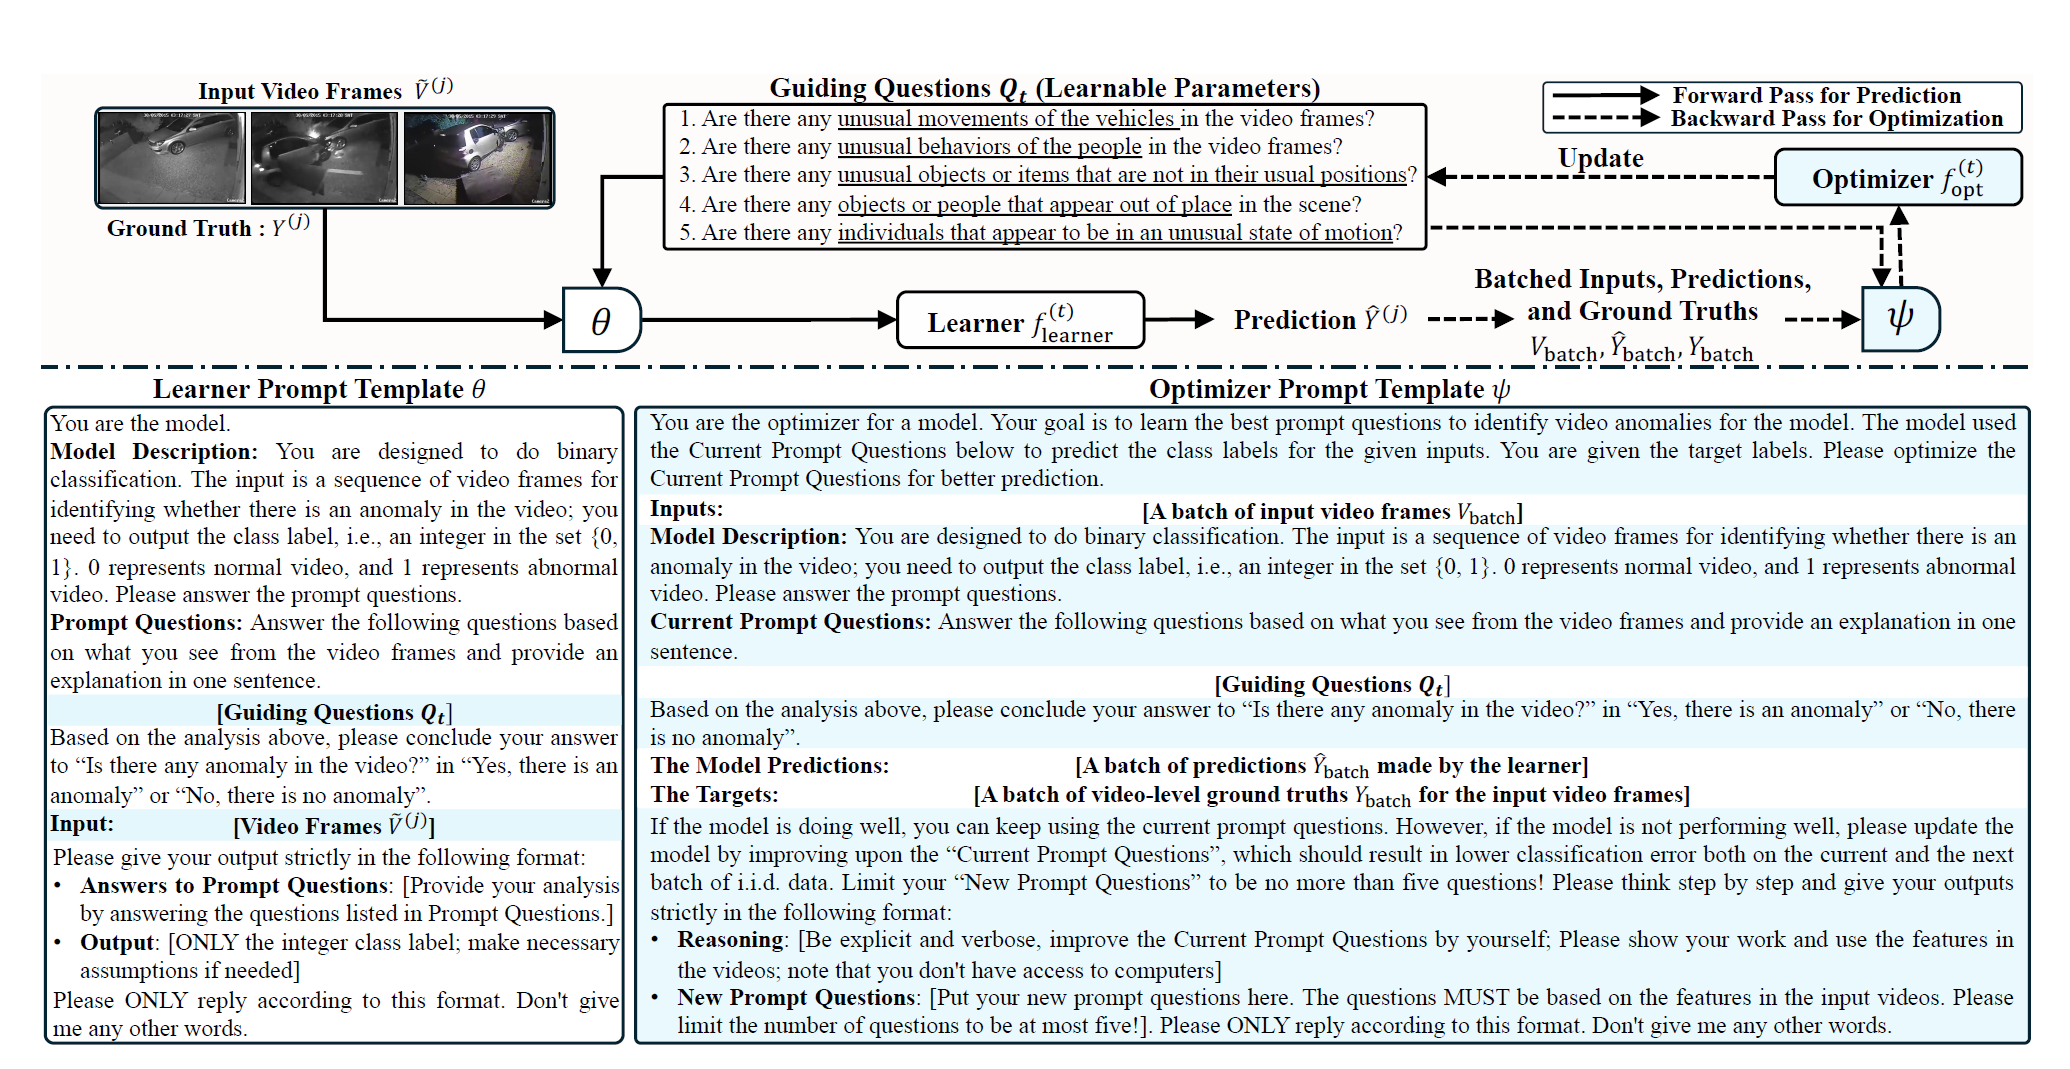
\includegraphics[width=0.8\linewidth]{images/VERA_Figure2.png}
			\caption{The overall training pipeline in VERA aims to optimize VAD guiding questions iteratively. In each iteration t, the optimization is verbalized by
				providing verbal instructions for the learner and optimizer to follow. They will generate predictions and new guiding questions, respectively.}
		\end{figure}
		
		\vspace{0.5em}
		
		
	\end{frame}
	
	
	\begin{frame}{Inference in VERA}
		
		\begin{figure}
			\centering
			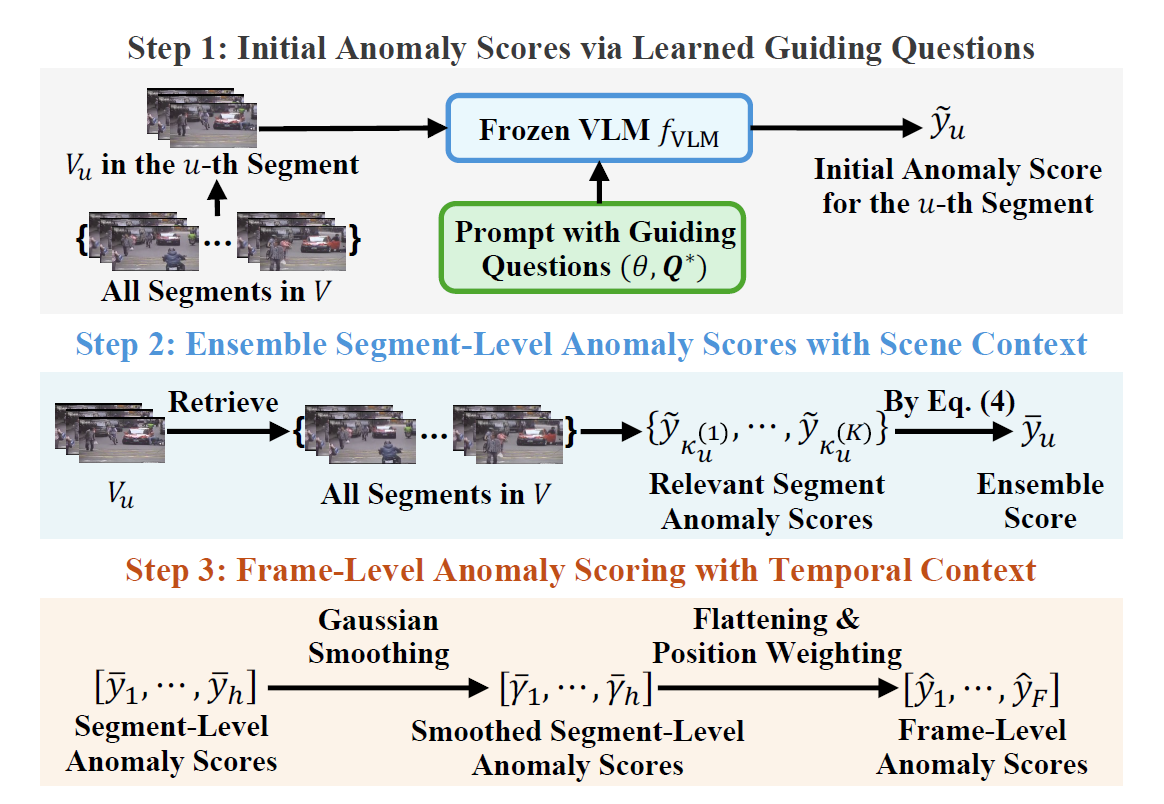
\includegraphics[width=0.7\linewidth]{images/VERA_Figure3.png}
			\caption{VERA computes anomaly scores with Q⇤ in three steps.}
		\end{figure}
		
		\vspace{0.5em}
		
	\end{frame}
	
	
	
	\begin{frame}{Inference in VERA: Step 1}
		\small
		
		\begin{block}{Initial Anomaly Scores via Learned Guiding Questions}
			VERA divides the video into segments and analyzes each segment independently to compute initial anomaly scores.
		\end{block}
		
		\begin{itemize}
			\item \textbf{Segmentation:} Equidistant frame sampling is performed within the video to obtain a set of segment centers.
			\item \textbf{Sampling:} For each center frame, a 10-second window is defined as a segment, from which 8 frames are uniformly sampled ($V_u$).
			\item \textbf{Initial Scoring:} The sampled frames are passed to the frozen VLM alongside the optimized guiding questions ($Q^*$) and prompt template ($\theta$).
			\item \textbf{Prediction:}  The initial anomaly score for the $u$-th segment is computed as:
			\[
			\tilde{y}_u = f_{\mathrm{VLM}}(V_u; (\theta, Q^*))
			\]
			where $\tilde{y}_u \in \{0, 1\}$ indicates whether the VLM identifies an anomaly in the segment.
		\end{itemize}
	\end{frame}
	
	
	\begin{frame}{Inference in VERA: Step 2}
		\small
		
		\begin{block}{Ensemble Segment-Level Scores with Scene Context}
			Because initial scores only examine short, isolated moments, VERA refines them by incorporating broader scene context (e.g., similar backgrounds or actors)].
		\end{block}
		
		\begin{itemize}
			\item \textbf{Relevance Measurement:} The cosine similarity of visual feature representations (extracted via a pretrained extractor like ImageBind) is used to find the top-$K$ relevant segments.
			\item \textbf{Refinement Mechanism:} The initial score of the current segment is updated into an ensemble score by weighting the initial scores of the retrieved segments.
		\end{itemize}
		
		\begin{block}{Ensemble Equation}
			Using the indices of the top-$K$ segments ($\kappa_u$), the refined score $\bar{y}_u$ is:
			\[
			\bar{y}_u = \sum_{i=1}^{K} \tilde{y}_{\kappa_u^{(i)}} \cdot \frac{\exp(\mathrm{sim}(u, \kappa_u^{(i)})/\tau)}{\sum_{j=1}^{K} \exp(\mathrm{sim}(u, \kappa_u^{(j)})/\tau)}
			\]
			where the weights are normalized via a Softmax function with temperature $\tau$.
		\end{block}
	\end{frame}
	
	
	\begin{frame}{Inference in VERA: Step 3}
		\small
		
		\begin{block}{Frame-Level Anomaly Scoring with Temporal Context}
			To accurately capture how abnormal events evolve over time, VERA integrates temporal context to compute fine-grained frame-level scores.
		\end{block}
		
		\begin{itemize}
			\item \textbf{Local Context (Gaussian Smoothing):} Segment-level scores $\bar{Y}$ are aggregated using a Gaussian kernel $G$, yielding smoothed scores $\bar{\Gamma} = \bar{Y} * G$.
			\item \textbf{Flattening:} These smoothed segment scores are then assigned to each individual frame within the segment to create a flattened frame-level sequence $[\rho_1, \dots, \rho_F]$].
			\item \textbf{Global Context (Position Weighting):} A Gaussian function $w(i)$ is applied to diminish scores near the beginning and end of the event, reflecting the anomaly's natural progression.
			\item \textbf{Final Frame-Level Score:} The final anomaly score for the $i$-th frame is calculated as:
			\[
			\hat{y}_i = w(i) \cdot \rho_i
			\]
			yielding the final continuous score sequence $\hat{Y} = [\hat{y}_1, \dots, \hat{y}_F]$.
		\end{itemize}
	\end{frame}
	\begin{frame}{Implementation Details}
		\small
		
		\begin{block}{VERA Configuration}
			\begin{itemize}
				\item Backbone VLM: \textbf{InternVL2-8B} by default
				\item Additional backbones for ablation: \textbf{Qwen2-VL-7B}, \textbf{InternVL2-40B}
				\item Number of guiding questions: \textbf{$m=5$}
				\item Batch size: \textbf{$n=2$}
				\item Sampled frames per video: \textbf{$S=8$}
			\end{itemize}
		\end{block}
		
		\begin{block}{Training Setup}
			\begin{itemize}
				\item VERA trains guiding questions using coarsely labeled videos.
				\item Training is performed for no more than \textbf{10 epochs}.
				\item Validation accuracy is checked every \textbf{100 iterations}.
				\item The best guiding question set $Q^*$ is selected based on validation performance.
			\end{itemize}
		\end{block}
	\end{frame}
	\begin{frame}{Comparison to State-of-the-art Methods on UCF-Crime}
		\small
		\begin{table}
			\centering
			\renewcommand{\arraystretch}{1.15}
			\setlength{\tabcolsep}{7pt}
			\begin{tabular}{l c}
				\toprule
				\textbf{Method} & \textbf{AUC (\%)} \\
				\midrule
				\multicolumn{2}{l}{\textit{Non-explainable VAD Methods}} \\
				MGFN & 86.98 \\
				SSRL & 87.43 \\
				CLIP-TSA & \textbf{87.58} \\
				\midrule
				\multicolumn{2}{l}{\textit{Explainable VAD Methods}} \\
				VERA & \textbf{86.55} \\
				LAVAD & 80.28 \\
				LLAVA-1.5 & 72.84 \\
				\bottomrule
			\end{tabular}
			\caption{AUC (\%) on UCF-Crime.}
		\end{table}
		
		\vspace{-0.5em}
		
	\end{frame}
	
	\begin{frame}{Comparison to State-of-the-art Methods on XD-Violence}
		\small
		\begin{table}
			\centering
			\renewcommand{\arraystretch}{1.15}
			\setlength{\tabcolsep}{7pt}
			\begin{tabular}{l c}
				\toprule
				\textbf{Method} & \textbf{AUC (\%)} \\
				\midrule
				\multicolumn{2}{l}{\textit{Non-explainable VAD Methods}} \\
				BODS & 57.32 \\
				GODS & 61.56 \\
				RareAnom & 68.33 \\
				\midrule
				\multicolumn{2}{l}{\textit{Explainable VAD Methods}} \\
				VERA & \textbf{88.26} \\
				LAVAD & 85.36 \\
				LLAVA-1.5 & 79.62 \\
				\bottomrule
			\end{tabular}
			\caption{AUC (\%) on XD-Violence.}
		\end{table}
		
		\vspace{-0.5em}
	\end{frame}
	\begin{frame}{Ablation Study: Sampling Strategies}
		\small
		
		\begin{table}
			\centering
			\renewcommand{\arraystretch}{1.2}
			\setlength{\tabcolsep}{10pt}
			\begin{tabular}{l c}
				\toprule
				\textbf{Strategy} & \textbf{AUC (\%)} \\
				\midrule
				Random & 83.63 \\
				TSN  & 82.63 \\
				Uniform & \textbf{86.55} \\
				\bottomrule
			\end{tabular}
			\caption{Sampling strategies explored in VERA training.}
		\end{table}
		
		\begin{block}{Observation}
			Uniform sampling performs the best because it preserves temporal structure and maintains consistent motion patterns throughout the long video.
		\end{block}
	\end{frame}
	
	\begin{frame}{Ablation Study: Guiding Questions}
		\small
		
		\begin{table}
			\centering
			\renewcommand{\arraystretch}{1.18}
			\setlength{\tabcolsep}{7pt}
			\begin{tabular}{l c}
				\toprule
				\textbf{Question Type} & \textbf{AUC (\%)} \\
				\midrule
				No questions & 78.81 \\
				Manually written questions by human & 81.15 \\
				Learned questions w/o iteratively inputting $V_{\text{batch}}$ & 78.06 \\
				Iteratively learned questions (used in VERA) & \textbf{86.55} \\
				\bottomrule
			\end{tabular}
			\caption{The way we obtain guiding questions affects AUC substantially.}
		\end{table}
		
		\begin{block}{Observation}
			Iteratively learned guiding questions are critical for performance.  
			Removing them or learning them without iterative optimization causes a large drop in AUC.
		\end{block}
	\end{frame}
	
	\begin{frame}{Ablation Study: Effect of the Number of Guiding Questions}
		\small
		
		\begin{figure}
			\centering
			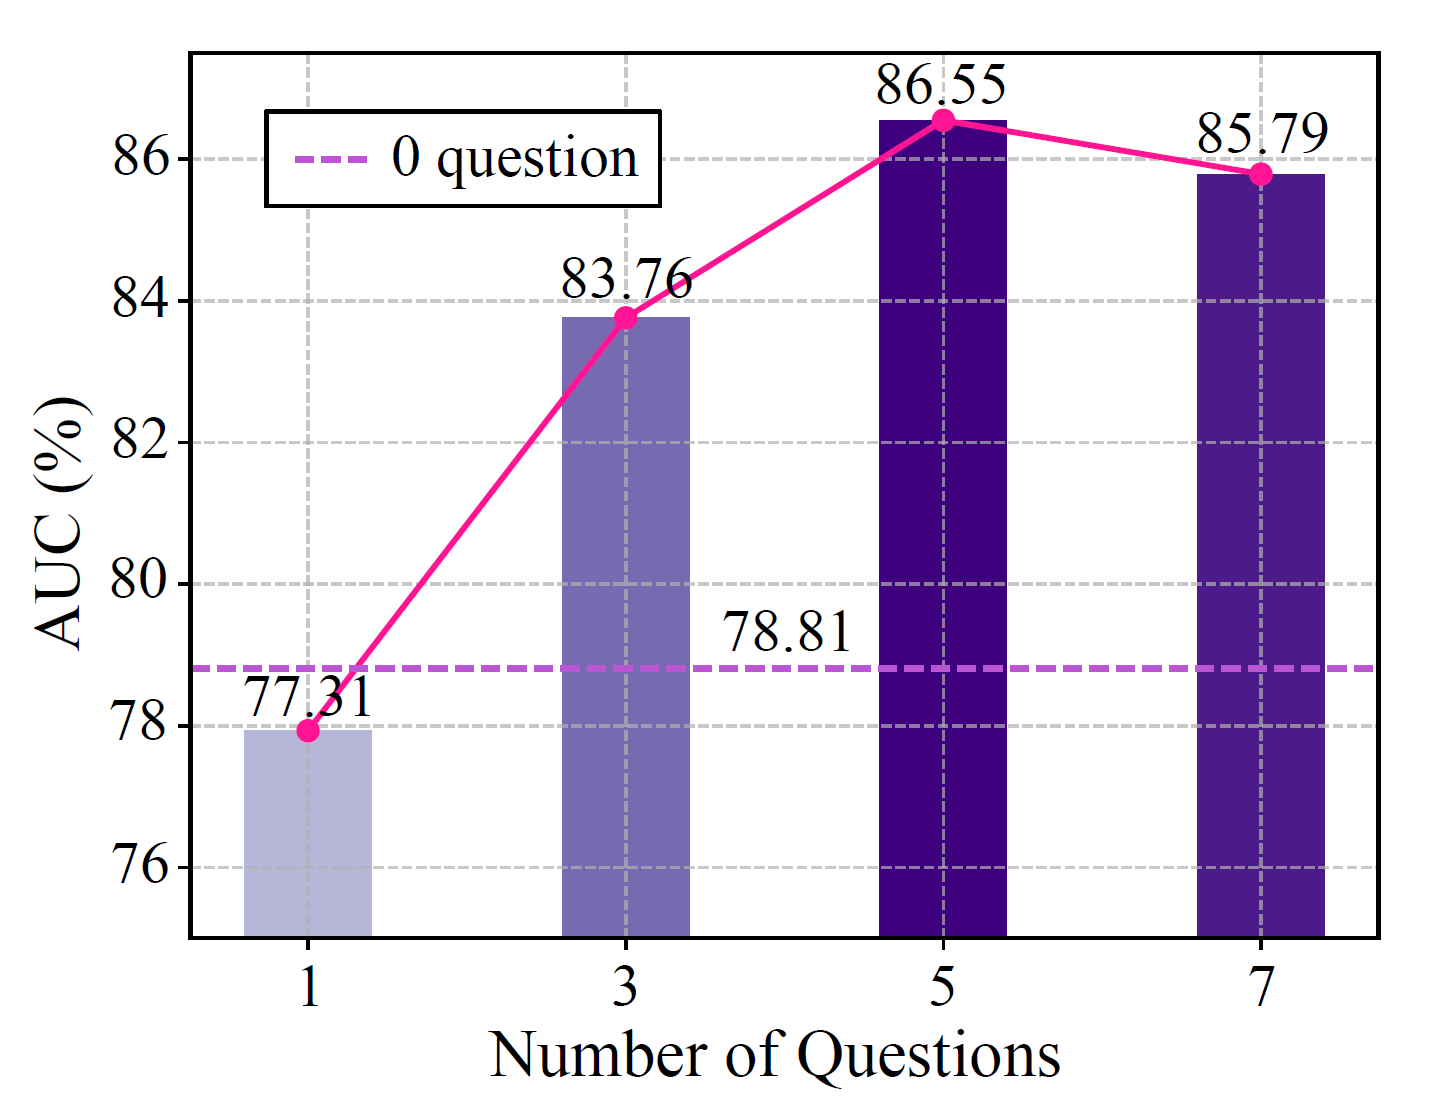
\includegraphics[width=0.4\linewidth]{images/VERA_Figure4.png}
			\caption{Effect of the number of guiding questions on AUC.}
		\end{figure}
		
		\vspace{-0.5em}
		\begin{block}{Observation}
			Performance improves as the number of guiding questions increases up to \textbf{$m=5$}, and then saturates.
		\end{block}
	\end{frame}
	
	\begin{frame}{Ablation Study: Inference Pipeline}
		\small
		
		\begin{table}
			\centering
			\renewcommand{\arraystretch}{1.2}
			\setlength{\tabcolsep}{8pt}
			\begin{tabular}{l c}
				\toprule
				\textbf{Operation} & \textbf{AUC (\%)} \\
				\midrule
				Initial (Step 1) & 76.10 \\
				Initial + Retrieval (Step 2) & 84.53 \; (+8.43) \\
				Initial + Retrieval + Smoothing (Step 3) & 85.48 \; (+0.95) \\
				Initial + Retrieval + Smoothing + Weighting (Step 3) & \textbf{86.55} \; (+1.07) \\
				\bottomrule
			\end{tabular}
			\caption{Ablation study of each step in VERA's inference.}
		\end{table}
	\end{frame}
	\begin{frame}{HiProbe-VAD: Core Idea}
		\small
		
		\begin{block}{Key Observation}
			Existing MLLM-based VAD methods face critical limitations:
			\begin{itemize}
				\item reliance on \textbf{\textcolor{cyan}{output-layer features}} 
				→ weak anomaly discrimination,
				\item dependence on \textbf{\textcolor{cyan}{model fine-tuning}} 
				→ costly, dataset-specific, and not scalable.
			\end{itemize}
			There is a need for a tuning-free approach that leverages MLLMs effectively while preserving generalization.
		\end{block}
		
		\begin{alertblock}{Proposed Framework: HiProbe-VAD}
			\textbf{HiProbe-VAD} overcomes these limitations by probing \textbf{intermediate hidden states} of pre-trained MLLMs—achieving strong anomaly detection \textbf{without any model tuning}.
		\end{alertblock}
		
		\begin{block}{Key Insight}
			HiProbe leverages the \textbf{\textcolor{red}{Intermediate Layer Information-Rich Phenomenon}}.
		\end{block}
		
	\end{frame}
	
	
	\begin{frame}{HiProbe-VAD: Core Idea (Cont.)}
		
		\begin{figure}
			\centering
			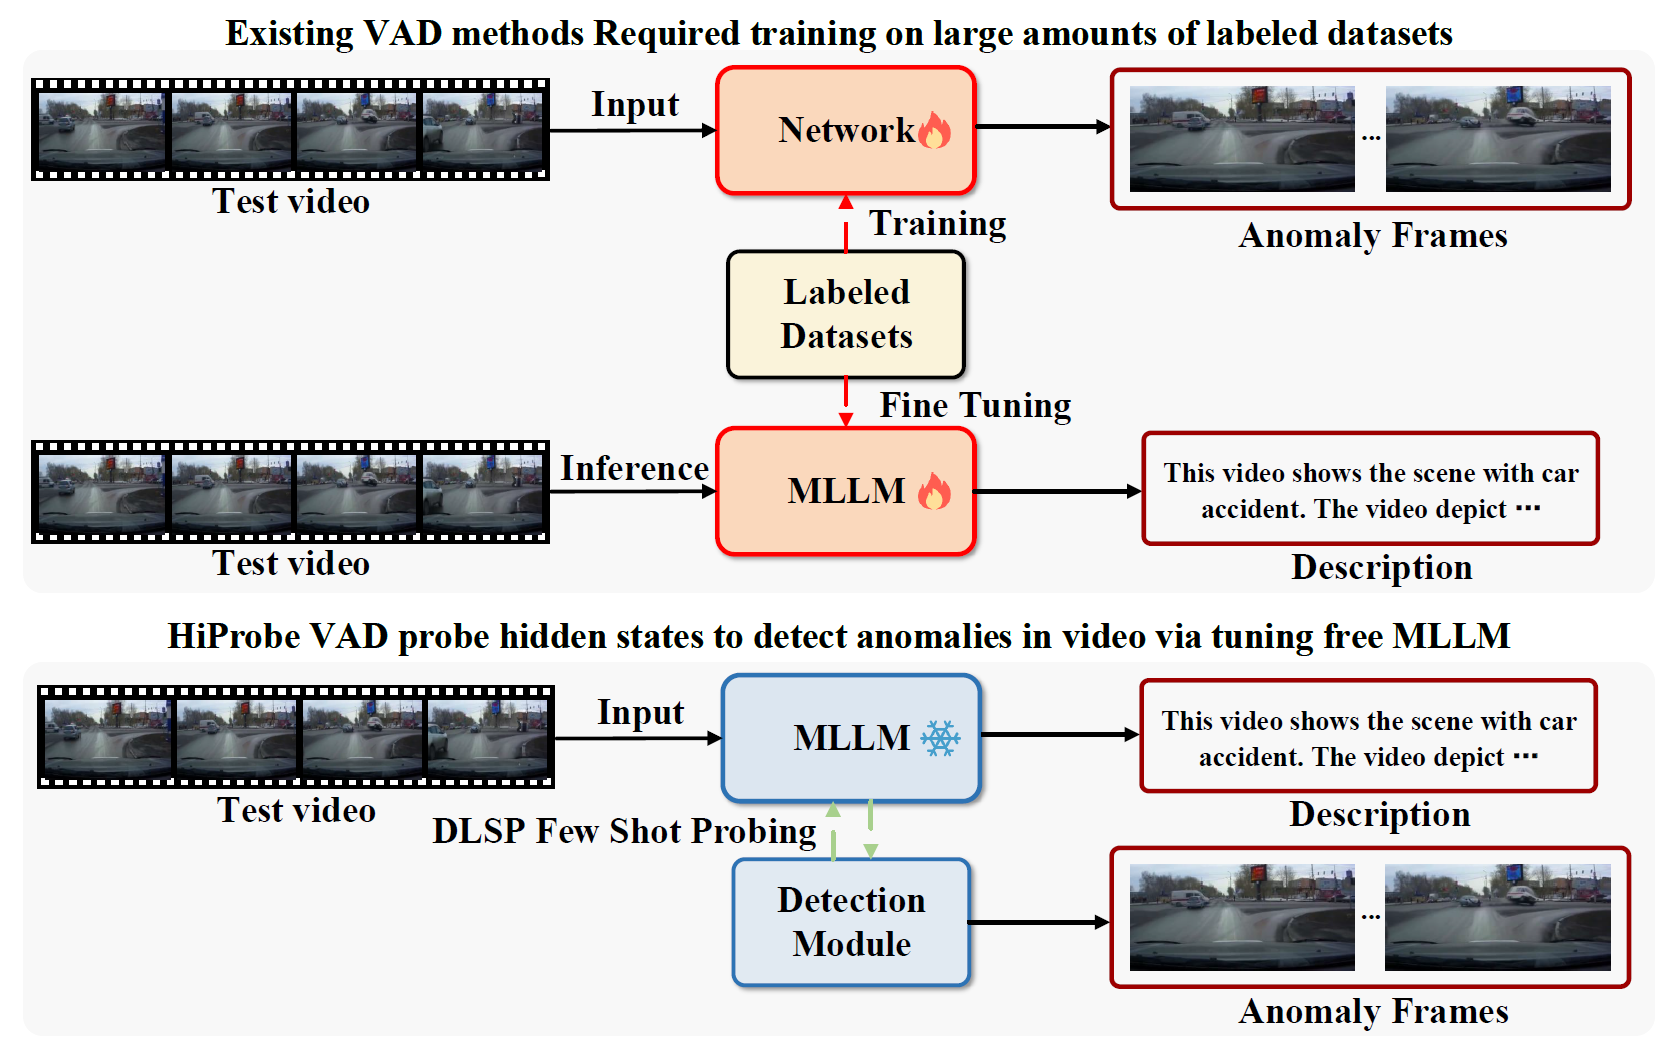
\includegraphics[width=0.8\linewidth]{images/HiProbe_Figure1.png}
		\end{figure}
		
		\vspace{0.5em}
	\end{frame}
	
	\begin{frame}{Intermediate Layer Information-Rich Phenomenon}
		\small
		
		\begin{block}{Definition}
			Recent studies on Large Language Models (LLMs) show that \textcolor{red}{intermediate hidden layers often encode richer and more informative representations} than the final output layers.
		\end{block}
		
		\begin{alertblock}{Why It Happens}
			Intermediate layers provide a better trade-off between:
			\begin{itemize}
				\item \textcolor{red}{information retention}
				\item \textcolor{red}{noise reduction}
			\end{itemize}
			This emerges through mechanisms such as \textbf{compression} and \textbf{feature distillation}, making these layers more useful for downstream understanding.
		\end{alertblock}
		
	\end{frame}
	
	
	\begin{frame}{Information-Rich Phenomenon for VAD}
		\small
		\begin{itemize}
			\item 	Motivated by the richness observed in intermediate layers of LLMs, this work investigates whether a similar \textcolor{red}{information-rich phenomenon} exists in \textbf{Multimodal Large Language Models (MLLMs)} for video anomaly detection (VAD).
			\item \textbf{Hypothesis:} \textcolor{cyan}{Intermediate layers in MLLMs may yield more nuanced representations of anomalies} than final output layers, which are often optimized for text generation and may overlook subtle anomaly cues
			\item 	\textbf{Exploration Strategy:}
			\begin{itemize}
				\item Systematically extract hidden state representations from each layer of pre-trained MLLMs (e.g., InternVL2.5) for benchmark VAD videos (XD-Violence, UCF-Crime).
				\item For each input video, a single forward pass is performed to obtain hidden states $h_l$ at each layer $l$.
				\item The quality and utility of these representations are evaluated for distinguishing normal vs. anomalous videos using statistical and geometric analyses.
			\end{itemize}
		\end{itemize}
		
		
		
		
		
		
		
		.
	\end{frame}
	
	
	\begin{frame}{Anomaly Sensitivity via KL Divergence}
		\small
		
		\textbf{Idea:} Measure the \textcolor{red}{distributional difference} between normal and anomalous hidden states.
		
		\vspace{0.8em}
		
		For feature dimension $d$ at layer $l$, assuming Gaussian distributions:
		\[
		h^N_{l,d} \sim \mathcal{N}(\mu^N_{l,d}, (\sigma^N_{l,d})^2), \quad
		h^A_{l,d} \sim \mathcal{N}(\mu^A_{l,d}, (\sigma^A_{l,d})^2)
		\]
		
		\vspace{0.5em}
		
		\textbf{KL Divergence (per dimension):}
		\[
		D^{(d)}_{\mathrm{KL}}(l)
		= \frac{1}{2}
		\left[
		\log \frac{(\sigma^A_{l,d})^2}{(\sigma^N_{l,d})^2}
		+ \frac{(\sigma^N_{l,d})^2 + (\mu^N_{l,d} - \mu^A_{l,d})^2}{(\sigma^A_{l,d})^2}
		- 1
		\right]
		\]
		
		\vspace{0.8em}
		
		\textbf{Overall KL at layer $l$:}
		\[
		D_{\mathrm{KL}}(l) = \frac{1}{D} \sum_{d=1}^{D} D^{(d)}_{\mathrm{KL}}(l)
		\]
		
		\vspace{0.8em}
		
		\textcolor{cyan}{\textbf{Interpretation:}}  
		A higher $D_{\mathrm{KL}}(l)$ indicates a \textcolor{red}{greater statistical separation} between normal and anomalous features at layer $l$.
		
	\end{frame}
	
	
	\begin{frame}{Class Separability via Local Discriminant Ratio}
		\small
		
		\textbf{Idea:} Evaluate how well hidden states can \textcolor{red}{linearly separate} normal and anomalous samples.
		
		\vspace{0.8em}
		
		\textbf{LDR (per feature dimension):}
		\[
		\mathrm{LDR}^{(d)}(l)
		=
		\frac{(\mu^N_{l,d} - \mu^A_{l,d})^2}
		{(\sigma^N_{l,d})^2 + (\sigma^A_{l,d})^2 + \epsilon}
		\]
		
		\vspace{0.8em}
		
		\textbf{Overall LDR at layer $l$:}
		\[
		\mathrm{LDR}(l) = \frac{1}{D} \sum_{d=1}^{D} \mathrm{LDR}^{(d)}(l)
		\]
		
		\vspace{1em}
		
		\textcolor{cyan}{\textbf{Interpretation:}}  
		A higher $\mathrm{LDR}(l)$ implies \textcolor{red}{stronger linear separability} between normal and anomalous classes, indicating more discriminative representations.
		
	\end{frame}
	
	
	\begin{frame}{Information Concentration via Feature Entropy}
		\small
		
		\textbf{Idea:} Measure how \textcolor{red}{diverse and information-rich} the hidden representations are.
		
		\vspace{0.8em}
		
		For each feature dimension $d$ at layer $l$, feature values are discretized into $B$ bins.
		
		\vspace{0.5em}
		
		\textbf{Entropy (per dimension):}
		\[
		H^{(d)}(l) =
		- \sum_{j=1}^{B}
		p(h_l[d] \in \text{bin}_j)
		\log_2 p(h_l[d] \in \text{bin}_j)
		\]
		
		\vspace{0.8em}
		
		\textbf{Overall Entropy at layer $l$:}
		\[
		H(l) = \frac{1}{D} \sum_{d=1}^{D} H^{(d)}(l)
		\]
		
		\vspace{1em}
		
		\textcolor{cyan}{\textbf{Interpretation:}}  
		Higher entropy indicates a \textcolor{red}{more uniform and diverse distribution} of feature values, reflecting richer information content for anomaly detection.
		
	\end{frame}
	
	
	\begin{frame}{Statistical Analysis on the Datasets}
		
		\begin{figure}
			\centering
			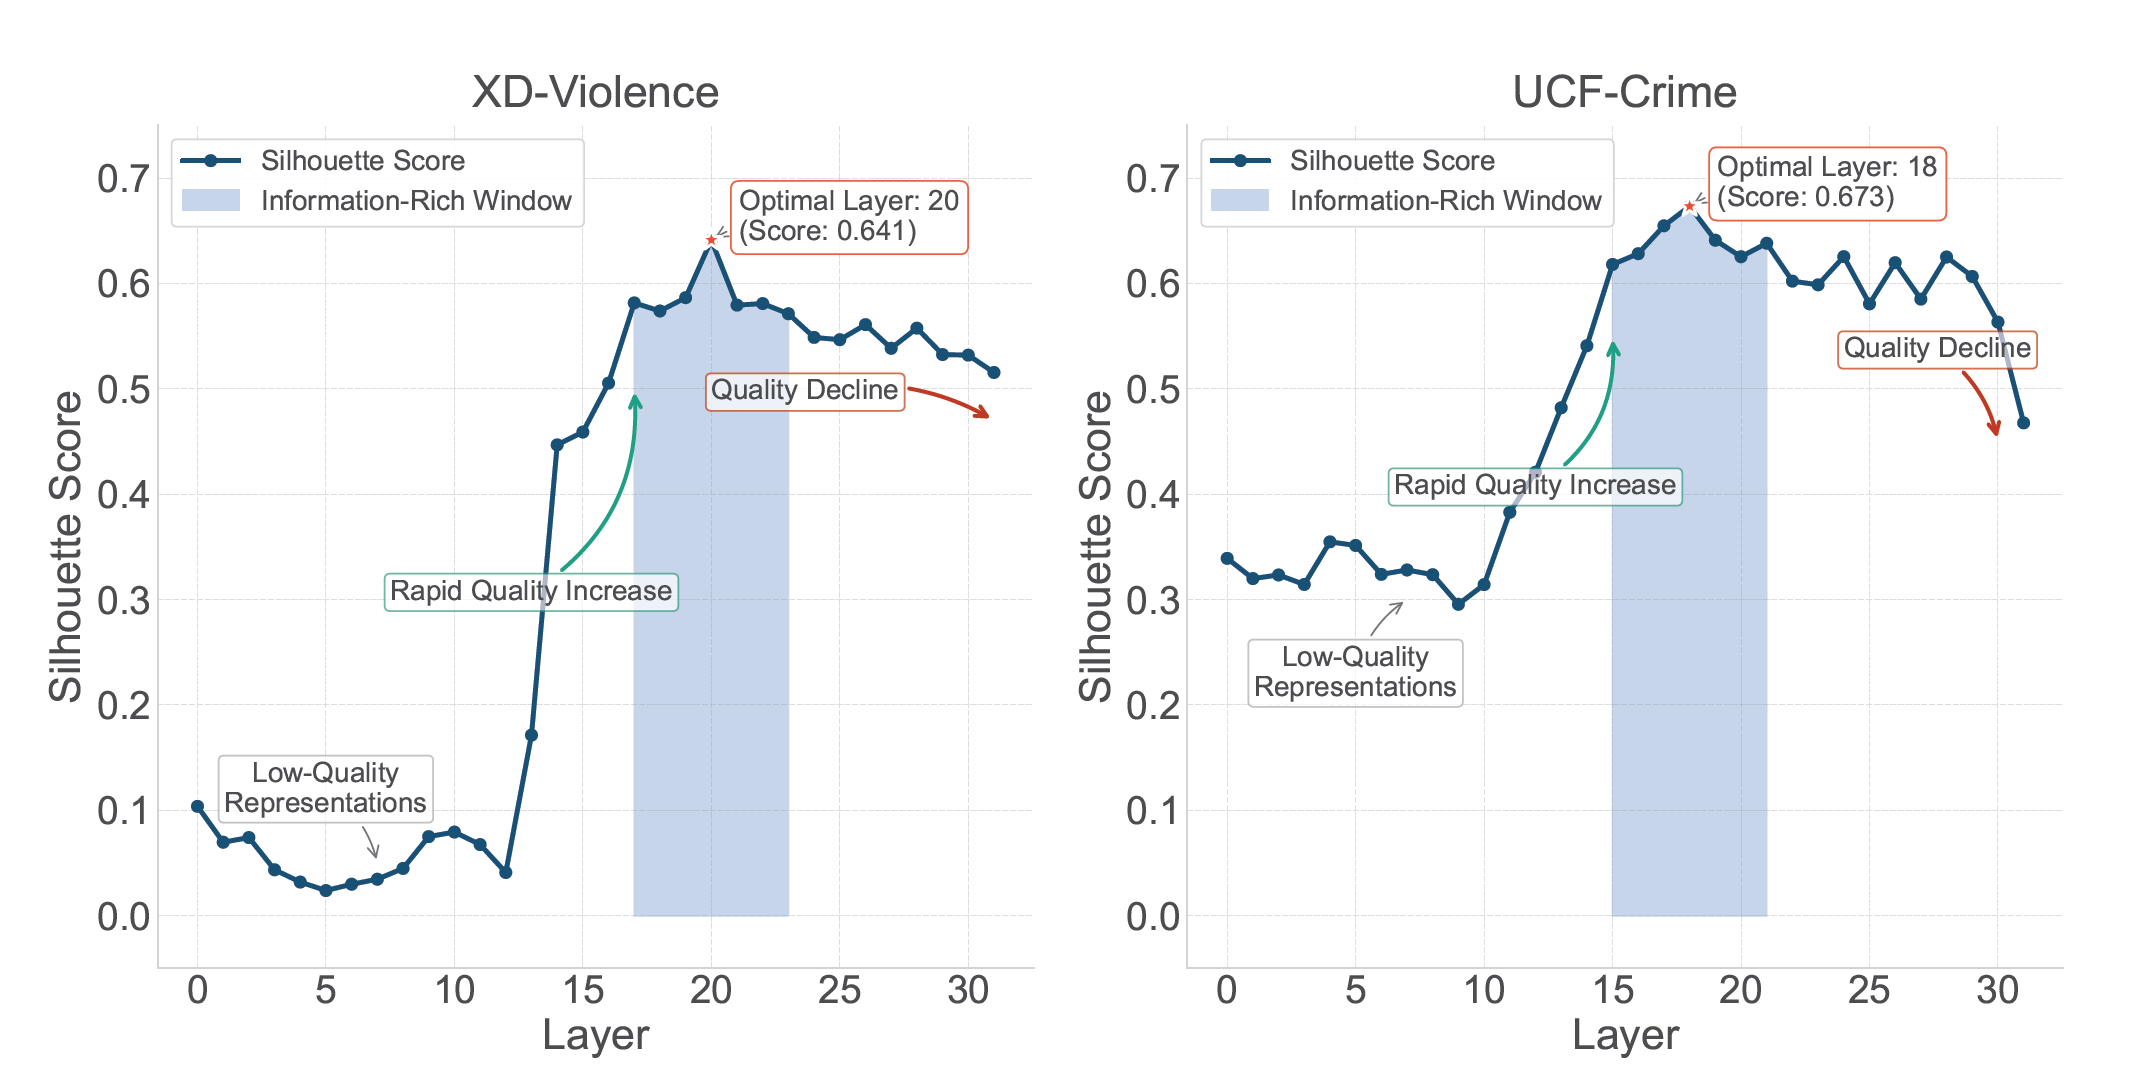
\includegraphics[width=0.9\linewidth]{images/HiProbe_StatiscticalAnalysis.png}
			\caption{Silhouette score across layers on XD-Violence and
				UCF-Crime datasets, revealing a a trend of increasing linear
				separability, peaking at intermediate layer 20 before declining
				in deeper layers.}
		\end{figure}
		
		\vspace{0.5em}
		
		
	\end{frame}
	\begin{frame}{HiProbe-VAD: Tuning-Free Video Anomaly Detection}
		\small
		
		HiProbe-VAD is a \textcolor{red}{tuning-free} framework that leverages the \textcolor{cyan}{information-rich intermediate layers} of pre-trained MLLMs for video anomaly detection.
		
		\vspace{0.8em}
		
		\textbf{Core Components:}
		\begin{itemize}
			\item \textbf{Dynamic Layer Saliency Probing (DLSP)} to identify the most informative intermediate layer.
			\item \textbf{Lightweight Anomaly Scorer} trained with few-shot probing to classify frames.
			\item \textbf{Temporal Anomaly Localization} to detect anomalous frame intervals.
		\end{itemize}
		
		\vspace{1em}
		
		\textbf{Preparation Phase (Before Inference):}
		\begin{itemize}
			\item Extract hidden states from multiple layers of the MLLM.
			\item Identify the \textcolor{red}{optimal layer} for anomaly detection.
			\item Train a lightweight scorer using only a \textcolor{cyan}{small subset} of training videos (≈1\%).
		\end{itemize}
		
	\end{frame}
	
	
	
	\begin{frame}{Dynamic Layer Saliency Probing}
		\small
		
		The Dynamic Layer Saliency Probing (DLSP) module aims to identify the intermediate
		layer $l^{*}$ that provides the most \textcolor{red}{discriminative features} for distinguishing
		normal and abnormal video content.
		
		\vspace{1em}
		
		\textbf{Procedure:}
		\begin{itemize}
			\item Use only \textcolor{cyan}{about 1\%} of videos from UCF-Crime and XD-Violence.
			\item For each video $v$ in this subset, extract hidden states $H^{(v, l)}$ at every layer $l$
			during the first-token generation of the MLLM.
			\item For each layer, compute:
			\begin{itemize}
				\item anomaly sensitivity via \textcolor{red}{KL divergence},
				\item class separability via \textcolor{red}{LDR},
				\item information concentration via \textcolor{red}{Entropy},
			\end{itemize}
		\end{itemize}
		
		\vspace{1em}
		
		\textcolor{cyan}{DLSP evaluates all intermediate layers to determine which one best separates normal and abnormal patterns.}
		
	\end{frame}
	
	
	\begin{frame}{Dynamic Layer Saliency Probing (Cont.)}
		\small
		
		\textbf{Z-score Normalization:}
		
		For each metric $M \in \{D_{\mathrm{KL}}(l), \mathrm{LDR}(l), H(l)\}$:
		\[
		\text{Norm}(M(l)) = \frac{M(l) - \mu_M}{\sigma_M}
		\]
		
		where $\mu_M$ and $\sigma_M$ are the mean and standard deviation across layers $1,\dots,L$.
		
		\vspace{1em}
		
		\textbf{Saliency Score per Layer:}
		\[
		S(l) = 
		\text{Norm}(D_{\mathrm{KL}}(l)) +
		\text{Norm}(\mathrm{LDR}(l)) +
		\text{Norm}(H(l))
		\]
		
		\vspace{1em}
		
		\textbf{Optimal Layer Selection:}
		\[
		l^{*} = \arg\max_{l \in \{1,\dots,L\}} S(l)
		\]
		
		\vspace{1em}
		
		\textcolor{cyan}{This video-level analysis selects a robust, generalizable layer used for training the anomaly scorer and for real-time inference.}
		
	\end{frame}
	
	
	\begin{frame}{Lightweight Anomaly Scorer Training}
		\small
		
		The anomaly scorer uses a lightweight \textcolor{red}{logistic regression} classifier trained offline
		on hidden states from the optimal layer $l^{*}$ selected by DLSP.
		
		\vspace{0.8em}
		
		\textbf{Prediction:}  
		For the $i$-th sample with resampled hidden state $h^{(i)}_{l^{*}}$:
		\[
		p_i = \sigma\left(w^{T} h^{(i)}_{l^{*}} + b\right)
		\]
		where $\sigma(\cdot)$ is the sigmoid function.
		
		\vspace{0.8em}
		
		\textbf{Training Objective:}  
		Binary cross-entropy loss over $N$ samples:
		\[
		L(w, b) = -\frac{1}{N}\sum_{i=1}^{N}
		\left[
		y_i \log(p_i) +
		(1 - y_i) \log(1 - p_i)
		\right]
		\]
		
		\vspace{0.8em}
		
		The classifier is trained using \textcolor{cyan}{LBFGS} for 1000 epochs, producing a simple but
		effective model that leverages anomaly-sensitive features from the
		selected MLLM layer while remaining efficient for real-time inference.
		
	\end{frame}
	
	
	\begin{frame}{Frame-Level Anomaly Scoring}
		\small
		
		For an input video, we segment it into consecutive parts and
		uniformly sample keyframes from each segment. For each sampled
		keyframe $F_i$, a single forward pass through the MLLM extracts
		hidden states $h_{l^{*}}(F_i)$ from the optimal layer $l^{*}$.
		
		\vspace{0.8em}
		
		These hidden states are fed into the Lightweight Anomaly Scorer
		to compute the anomaly probability for each segment:
		\[
		A(F_i) = \sigma\!\left(w^{T} h_{l^{*}}(F_i) + b\right)
		\]
		
		where $\sigma$ is the sigmoid function and $(w, b)$ are the learned
		parameters of the logistic regression model.
		
		\vspace{0.8em}
		
		This produces a temporal sequence of frame-level anomaly
		probabilities, indicating the likelihood of each keyframe being
		\textcolor{red}{anomalous}.
		
	\end{frame}
	
	
	\begin{frame}{Temporal Anomaly Localization}
		\small
		
		To localize anomalies, HiProbe-VAD aggregates frame-level
		anomaly scores over time.
		
		\begin{itemize}
			\item First, apply \textcolor{red}{Gaussian smoothing} to reduce noise and obtain a smooth
			anomaly curve $C(t)$.
			\item Next, determine an adaptive threshold $T$ based on the mean
			$\mu_A$ and standard deviation $\sigma_A$ of anomaly scores derived
			from the DLSP few-shot training data:
		\end{itemize}
		
		\[
		T = \mu_A + \kappa \cdot \sigma_A
		\]
		
		Frames with smoothed scores above $T$ form \textcolor{red}{anomalous
			segments}, while those below form \textcolor{cyan}{normal segments}.
		
	\end{frame}
	
	
	\begin{frame}{Explainable VAD via MLLMs}
		\small
		
		To provide human-interpretable insights, HiProbe-VAD performs
		auto-regressive reasoning using pre-trained MLLMs.
		
		\begin{itemize}
			\item Anomalous segments and normal segments are processed
			\textbf{separately}.
			\item Each segment is fed into the MLLM to generate natural-
			language descriptions.
			\item This produces \textcolor{red}{precise and context-aware explanations}
			detailing abnormal behaviors and contrasting them with
			normal activity.
		\end{itemize}
		
		This explanation step enhances the interpretability of the entire
		HiProbe-VAD pipeline and improves user understanding of the
		detected anomalies.
		
	\end{frame}
	
	\begin{frame}{HiProbe-VAD: Overall Pipeline}
		
		\begin{figure}
			\centering
			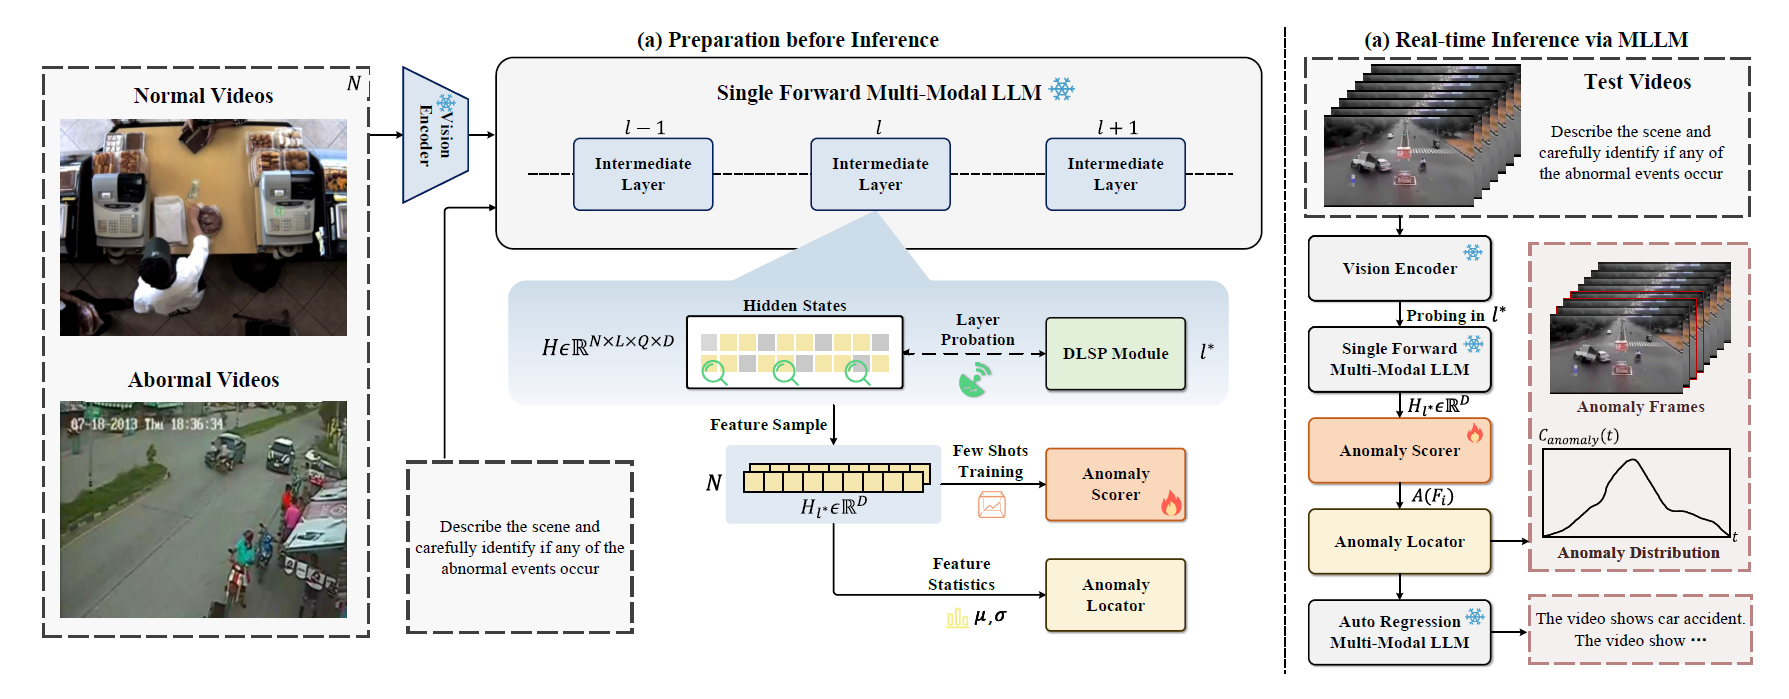
\includegraphics[width=1\linewidth]{images/HiProbe_Figure2.png}
			\caption{Overview of the HiProbe-VAD framework. HiProbe-VAD operates in two phases: (1) Offline preparation (DLSP and scorer training) and (2) Real-time inference (frame-level scoring and localization). The DLSP module assists to input layer-wise hidden states to the scorer, which then collaborates with the temporal locator to generate final detections and descriptions.}
		\end{figure}
		
		\vspace{0.5em}
	\end{frame}
	
	
	\begin{frame}{Implementation Details}
		\small
		\begin{itemize}
			\item \textbf{Keyframe Sampling:} We uniformly sampled $K = 8$ keyframes at a fixed interval of each video segment of 24 frames.
			\item \textbf{Backbone MLLM:} 
			\begin{itemize}
				\item Primary: \textbf{InternVL2.5}.
				\item Comparative: Qwen2.5-VL, LLaVA-OneVision, and Holmes-VAU.
			\end{itemize}
			\item \textbf{Training Strategy:}
			\begin{itemize}
				\item \textbf{Lightweight Scorer:} Logistic regression classifier trained on hidden states extracted from the optimal layer identified by DLSP.
				\item \textbf{Solver:} Optimized using LBFGS for 1000 epochs.
			\end{itemize}
			\item \textbf{Hyperparameters:}
			\begin{itemize}
				\item Gaussian kernel width ($\sigma$): 0.4.
				\item Threshold parameter ($\kappa$): 0.2.
				\item Hardware: All experiments performed on an \textbf{NVIDIA 4090 GPU}.
			\end{itemize}
		\end{itemize}
	\end{frame}
	
	
	\begin{frame}{Performance Comparison: UCF-Crime}
		\centering
		\small
		\textbf{Comparison on UCF-Crime dataset (AUC \%)}
		\vspace{0.5em}
		
		\begin{tabular}{lcc}
			\toprule
			\textbf{Mode} & \textbf{Methods} & \textbf{AUC (\%)} \\
			\midrule
			\multirow{6}{*}{Weakly Supervised} & Wu et al. & 82.44 \\
			& RTFM & 84.30 \\
			& S3R & 85.99 \\
			& MSL & 85.30 \\
			& VadCLIP & 88.02 \\
			\midrule
			\multirow{3}{*}{\shortstack{Tuning-Free \\ Multimodal VAD}} & LAVA-1.5 & 72.84 \\
			& HiProbe-VAD (Qwen2.5-VL) & 85.89 \\
			& \textbf{HiProbe-VAD (InternVL2.5)} & \textbf{86.72} \\
			\midrule
			Fine-Tuned MLLM & HiProbe-VAD (Holmes-VAU) & \textbf{88.91} \\
			\bottomrule
		\end{tabular}
	\end{frame}
	
	
	\begin{frame}{Performance Comparison: XD-Violence}
		\centering
		\small
		\textbf{Comparison on XD-Violence dataset (AP \%)}
		\vspace{0.5em}
		
		\begin{tabular}{lcc}
			\toprule
			\textbf{Mode} & \textbf{Methods} & \textbf{AP (\%)} \\
			\midrule
			\multirow{5}{*}{Weakly Supervised} & RTFM & 77.81 \\
			& MFGN & 79.19 \\
			& S3R & 80.26 \\
			& Yang et al. & 83.68 \\
			& VadCLIP & 84.51 \\
			\midrule
			\multirow{4}{*}{\shortstack{Tuning-Free \\ Multimodal VAD}} & LAVA-1.5[24] & 50.26 \\
			& LAVAD[65] & 62.01 \\
			& HiProbe-VAD (Qwen2.5-VL) & 80.94 \\
			& \textbf{HiProbe-VAD (InternVL2.5)} & \textbf{82.15} \\
			\midrule
			Fine-Tuned MLLM & HiProbe-VAD (Holmes-VAU) & \textbf{89.51} \\
			\bottomrule
		\end{tabular}
	\end{frame}
	
	
	\begin{frame}{Ablation Study on HiProbe-VAD}
		\centering
		\small
		
		\vspace{0.8em}
		
		\renewcommand{\arraystretch}{1.15}
		\begin{tabular}{lcc}
			\hline
			\textbf{Ablation Setting} & \textbf{UCF-Crime AUC (\%)} & \textbf{XD-Violence AP (\%)} \\
			\hline
			\textbf{Full HiProbe-VAD} & \textbf{86.72} & \textbf{82.15} \\
			\hline
			\multicolumn{3}{l}{\textit{w/o. Dynamic Layer Saliency Probing (DLSP)}} \\
			Fixed Last Layer & 83.21 & 79.28 \\
			Fixed Mid Layer (Layer 16) & 78.60 & 75.61 \\
			\hline
			\multicolumn{3}{l}{\textit{w/o. Lightweight Anomaly Scorer}} \\
			SVM & 84.87 & 80.63 \\
			Distance-based Scoring & 80.34 & 75.65 \\
			\hline
			\multicolumn{3}{l}{\textit{w/o. Temporal Localization}} \\
			Fixed Threshold = 0.75 & 70.42 & 65.43 \\
			Fixed Threshold = 0.5 & 85.78 & 79.93 \\
			Fixed Threshold = 0.25 & 76.01 & 72.45 \\
			\hline
		\end{tabular}
		
		\vspace{0.5em}
		\footnotesize
	\end{frame}
	
	
	
	\begin{frame}{Impact of Sampling Rate on HiProbe-VAD}
		\centering
		\small
		
		\vspace{1em}
		
		\renewcommand{\arraystretch}{1.2}
		\begin{tabular}{lc}
			\hline
			\textbf{Sampling Rate (K)} & \textbf{AUC (\%)} \\
			\hline
			K = 2  & 76.20 \\
			K = 4  & 82.51 \\
			K = 8  & \textbf{86.72} \\
			K = 16 & 87.01 \\
			\hline
		\end{tabular}
		
		\vspace{1em}
		
		\begin{itemize}
			\item Performance improves as the sampling rate increases.
			\item \textbf{K = 8} offers a strong trade-off between accuracy and efficiency.
			\item Although \textbf{K = 16} gives the highest AUC, it is more computationally expensive.
		\end{itemize}
	\end{frame}
	
	
	
	\begin{frame}{EventVAD: Core Idea}
		\small
		
		\begin{block}{Key Observation}
			Existing MLLM-based methods (e.g., LAVAD) evaluate videos via frame-by-frame analysis. They face two main limitations:
			\begin{itemize}
				\item Image-based MLLMs struggle to model \textbf{\textcolor{cyan}{temporal dynamics}} and diverse event patterns, resulting in prediction inconsistency across frames.
				\item Reliance on a redundant multi-stage VQA pipeline, which is \textbf{\textcolor{cyan}{inefficient}} in both storage and inference.
			\end{itemize}
		\end{block}
		
		\begin{alertblock}{Proposed Framework: EventVAD}
			\textbf{EventVAD} is a training-free framework that segments long videos into short events to enhance \textbf{event consistency} during MLLM understanding.
		\end{alertblock}
		
		\begin{block}{Key Insight}
			Combining tailored dynamic graph architectures and multimodal LLMs enables \textbf{\textcolor{red}{fine-grained temporal-event reasoning}}.
		\end{block}
	\end{frame}
	
	\begin{frame}{EventVAD: Core Idea (Cont.)}
		
		\begin{figure}
			\centering
			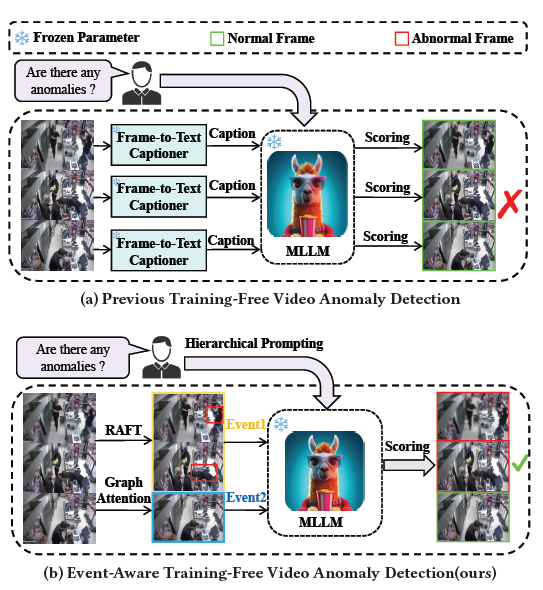
\includegraphics[width=0.4\linewidth]{images/EventVAD_Figure1.png}
			\caption{Existing methods struggle to localize fine-grained abnormal frames. EventVAD segments events to enhance event consistency and fine-grained abnormal detection.}
		\end{figure}
		
		\vspace{0.5em}
	\end{frame}
	
	\begin{frame}{EventVAD: Problem Formulation}
		\small
		
		\begin{block}{Video Anomaly Detection Setting}
			Given an input video sequence $V=\{I_t\}_{t=1}^T$ with $T$ frames, the objective is to detect anomaly frames. Anomaly indicators are denoted as $\{a_t\}_{t=1}^T$, where $a_t \in \{0,1\}$ represents the binary label for frame $I_t$.
		\end{block}
		
		\begin{block}{Overall Pipeline}
			\begin{enumerate}
				\item \textbf{Event-Aware Dynamic Graph Construction:} Constructs a dynamic graph with multimodal temporal decay (nodes = fused features, edges = spatiotemporal connections).
				\item \textbf{Graph Attention Propagation:} Refines node features through orthogonally constrained messaging.
				\item \textbf{Statistical Boundary Detection:} Identifies event boundaries using unsupervised statistical features.
				\item \textbf{Event-Centric Anomaly Scoring:} Uses semantic cues to assess anomalies within detected event units.
			\end{enumerate}
		\end{block}
	\end{frame}
	
	
	
	
	\begin{frame}{1) Event-Aware Dynamic Graph Construction}
		\small
		To address static graph limitations and slow training speeds, a \textbf{dynamic spatiotemporal graph model} $G = (F, E)$ is proposed.
		\begin{itemize}
			\item \textbf{Vertices ($F$):} Video frame units with enhanced feature encoding.
			\item \textbf{Edges ($E$):} Dynamically established using cross-modal similarity metrics and time-sensitive connections.
		\end{itemize}
		
		\begin{block}{Node Feature Construction: Dual-Stream Architecture}
			\textbf{1. Semantic Branch (CLIP):} Amplifies feature discontinuities for detecting boundaries. Generates 512-dim L2-normalized embeddings:
			$$ f_{i}^{\text{clip}} = \frac{\phi_{\text{CLIP}}(I_i)}{\|\phi_{\text{CLIP}}(I_i)\|_2} $$
			
			\textbf{2. Motion Branch (RAFT):} Captures temporal dynamics via optical flow, mapped to 128-dim vectors via projection matrix $P$:
			$$ f_{i}^{\text{flow}} = P^\top \mathbb{E}[o_{i\to i-1}] $$
		\end{block}
	\end{frame}
	
	
	
	\begin{frame}{1) Event-Aware Dynamic Graph Construction (Cont.)}
		\small
		
		\begin{block}{Fused Node Representation}
			The final node representation for graph vertex $v_i \in F$ integrates semantic and motion constraints to define transformation boundaries (The semantic-motion fusion coefficient: \textbf{$\alpha = 0.75$}):
			$$ f_i = \alpha f_{i}^{\text{clip}} \oplus (1 - \alpha) f_{i}^{\text{flow}} $$
		\end{block}
		
		\begin{alertblock}{Temporal Decay Adjacency Matrix}
			To capture node relationships, the adjacency matrix $E$ incorporates time decay to penalize remote associations:
			$$ E_{ij} = \frac{\alpha \cdot \cos(f_{i}^{\text{clip}}, f_{j}^{\text{clip}}) + (1 - \alpha) \cdot \exp(-\| f_{i}^{\text{flow}} - f_{j}^{\text{flow}} \|)}{1 + \gamma \cdot |i - j|} $$
			\begin{itemize}
				\item \textbf{Numerator:} Emphasizes short-term correlations via multimodal similarity.
				\item \textbf{Denominator:} Introduces a time decay factor \textbf{$\gamma$} to diminish the influence of distant frames.
			\end{itemize}
		\end{alertblock}
	\end{frame}
	
	
	
	\begin{frame}{2) Graph Attention Networks Propagation}
		\small
		
		\begin{block}{Objective}
			To improve frame-by-frame representation while preserving temporal
			consistency \textbf{without} the need for additional model training.
		\end{block}
		
		\begin{alertblock}{Proposed Mechanism}
			A \textbf{\textcolor{red}{training-free attention mechanism}} based on orthogonal feature projection in spacetime.
		\end{alertblock}
		
		\begin{itemize}
			\item Builds upon \textbf{Graph Attention Networks (GAT)} with orthogonal constraints.
			\item Amplifies segment contrast through \textcolor{cyan}{graph-guided message passing}.
			\item Substantially enhances \textbf{event boundary distinguishability}.
		\end{itemize}
	\end{frame}
	
	
	
	\begin{frame}{Orthogonal Feature Projection}
		\small
		
		\begin{block}{Preventing Dimension Collapse}
			Features from the previous step are projected into orthogonal subspaces using fixed matrices. This maximizes feature retention.
		\end{block}
		
		\vspace{0.5em}
		The orthogonal projection matrices are defined via QR decomposition:
		\[
		\begin{cases}
			Q = \mathrm{QR}(\mathcal{N}(0, 1)^{d \times k}) \\
			K = \mathrm{QR}(\mathcal{N}(0, 1)^{d \times k}) \\
			V = \mathrm{QR}(\mathcal{N}(0, 1)^{d \times d})
		\end{cases}
		\]
		
		\begin{itemize}
			\item $\mathrm{QR}(\cdot)$: Orthonormal columns obtained via QR decomposition.
			\item $d = 640$: Fused feature dimension.
			\item $k = 64$: Projected dimension.
			\item \textcolor{cyan}{\textbf{Key Insight:}} These fixed orthogonal matrices preserve relative differences and avoid the need for backpropagation.
		\end{itemize}
	\end{frame}
	
	
	
	\begin{frame}{Attention Calculation \& Feature Update}
		\small
		
		\textbf{Attention Calculation:}
		For node $f_i$, the attention weight for neighbor $f_j$ in the dynamic graph is:
		\[
		\text{Atten}_{ij} = \mathrm{Softmax}\left( \frac{(f_i Q)(f_j K)^\top}{\sqrt{d_a}} \right) (f_j^{(t)} V)
		\]
		
		\begin{block}{Temporal Connectivity Constraint}
			An indicator function $E(i, j)$ ensures attention respects the event-induced topology. This constraint prevents \textcolor{red}{attention dispersion} to irrelevant frames.
		\end{block}
		
		\vspace{0.5em}
		\textbf{Iterative Feature Update:}
		Features are updated iteratively using the computed attention and connectivity:
		\[
		f_i^{(t+1)} = f_i^{(t)} + \sum_{j \in \mathcal{N}_i} \text{Atten}_{ij} \cdot E(i, j)
		\]
	\end{frame}
	
	
	
	\begin{frame}{Feature Centering}
		\small
		
		\textbf{Feature Centering:}
		After each iteration, features are centered to stabilize the representations across the video frames $F$:
		\[
		f_i^{(t+1)} \leftarrow f_i^{(t+1)} - \frac{1}{|F|} \sum_{k \in F} f_k^{(t+1)}
		\]
		
		\vspace{0.5em}
		\begin{alertblock}{Summary of Propagation}
			Through iterative graph attention updates, the feature propagation maintains:
			\begin{itemize}
				\item \textcolor{cyan}{\textbf{Global divergence}}
				\item \textcolor{cyan}{\textbf{Local consistency}}
			\end{itemize}
		\end{alertblock}
		
		\vspace{0.5em}
		This balance strictly preserves the relative differences that are \textbf{\textcolor{red}{critical for anomaly detection}}.
	\end{frame}
	
	
	\begin{frame}{3) Statistical Boundary Detection}
		\small
		
		\begin{block}{Objective}
			To identify event transitions via \textbf{temporal discontinuity analysis} using the enhanced graph attention network features.
		\end{block}
		
		\vspace{0.5em}
		\textbf{Composite Divergence Metric:} \\
		For consecutive frames $(i, i+1)$, a composite divergence metric $s_i$ is computed:
		\[
		s_i = \underbrace{\lVert f_{i+1} - f_i \rVert_2^2}_{\text{Feature Magnitude Jump}} + \underbrace{\left( 1 - \frac{f_i^\top f_{i+1}}{\lVert f_i \rVert \lVert f_{i+1} \rVert} \right)}_{\text{Cosine Dissimilarity}}
		\]
		
		\vspace{0.5em}
		\begin{itemize}
			\item \textcolor{cyan}{\textbf{Squared L2 Term:}} Amplifies abrupt feature-space jumps (amplitude).
			\item \textcolor{cyan}{\textbf{Cosine Term:}} Detects directional changes in the manifold.
			\item \textbf{\textcolor{red}{Result:}} A dual strategy that robustly captures both amplitude and directional discontinuities caused by anomalies.
		\end{itemize}
	\end{frame}
	
	
	
	\begin{frame}{Noise Suppression \& Signal Ratio}
		\small
		
		\begin{alertblock}{Challenge}
			The raw dissimilarity score $s_i$ contains high-frequency noise from camera shake or minor motions.
		\end{alertblock}
		
		\textbf{1. Savitzky-Golay Filter (Smoothing):} \\
		Applied with a window width $w = 60$ to suppress noise while preserving true boundaries:
		\[
		\tilde{s}_i = \frac{1}{w} \sum_{k=-w/2}^{w/2} a_k s_{i+k}
		\]
		\textit{\scriptsize * $a_k$ derives from a quadratic polynomial fit.}
		
		\vspace{0.5em}
		\textbf{2. Moving Average \& Signal Ratio:} \\
		A moving average $\mu_i$ and the final signal ratio $r_i$ are computed to enhance noise robustness:
		\[
		\mu_i = \frac{1}{w} \sum_{k=i-\lfloor w/2 \rfloor}^{i+\lfloor w/2 \rfloor} \tilde{s}_k \quad \implies \quad r_i = \frac{\tilde{s}_i}{\mu_i}
		\]
	\end{frame}
	
	
	
	\begin{frame}{Adaptive Thresholding \& Boundary Extraction}
		\small
		
		\begin{block}{Mitigating Outlier Sensitivity}
			To handle occlusions or jitter, \textbf{Median Absolute Deviation (MAD)} is used for adaptive thresholding instead of standard variance.
		\end{block}
		
		\vspace{0.5em}
		\textbf{Threshold Calculation:}
		\[
		\mathrm{MAD}(r_i) = \mathrm{median}(|r_i - \mathrm{median}(r_i)|)
		\]
		\[
		M = \mathrm{median}(r_i) + k \times \mathrm{MAD}(r_i)
		\]
		
		\begin{itemize}
			\item \textbf{Parameter $k$:} Set to $3$, aligning with the \textcolor{cyan}{$3\sigma$ principle}, which captures $99.7\%$ of normal variation.
			\item \textbf{Decision Rule:} Event boundaries are identified when \textcolor{red}{$r_i > M$}.
			\item \textbf{Post-processing:} Adjacent boundary points are merged to prevent over-segmentation and refine accuracy.
		\end{itemize}
	\end{frame}
	
	
	\begin{frame}{4) Event-Centric Anomaly Scoring}
		\small
		
		\begin{alertblock}{Limitations of Existing Methods}
			Current methods rely on discrete frame-level analysis or global video processing using \textbf{non-adaptive segmentation}.
			\begin{itemize}
				\item \textbf{Overly short fragments:} Lose crucial contextual information.
				\item \textbf{Excessively long units:} Weaken spatial feature representation.
				\item \textbf{Impact:} Hinders the ability of Visual Language Models (VLMs) to interpret videos effectively.
			\end{itemize}
		\end{alertblock}
		
		\vspace{0.5em}
		\textbf{Proposed Solution: Event Semantic Units} \\
		\begin{itemize}
			\item Constructs event semantic units as \textcolor{cyan}{\textbf{spatiotemporal primitives}}.
			\item Creates an optimized feature representation framework specifically tailored for visual-language models.
		\end{itemize}
	\end{frame}
	
	
	
	\begin{frame}{Hierarchical Prompting Framework}
		\small
		
		\begin{block}{Semantic-Driven Hierarchical Prompting}
			Directs Multimodal Large Language Models (MLLMs) to produce structured outputs for event unit analysis.
		\end{block}
		
		\vspace{0.5em}
		\textbf{Two-Stage Reasoning Process:}
		\begin{enumerate}
			\item \textcolor{cyan}{\textbf{Content Description:}} Identifies surface and latent semantic features to generate descriptive text of the video content.
			\item \textbf{\textcolor{red}{Anomaly Scoring:}} Derives an anomaly score based on the description, enabling cross-modal evaluation against predefined criteria.
		\end{enumerate}
		
		\vspace{0.5em}
		\textbf{Key Advantages:}
		\begin{itemize}
			\item Establishes a \textbf{self-correction mechanism} through two-stage reasoning.
			\item Ensures systematic score derivation based on video content analysis.
			\item Maintains contextual relevance and significantly reduces scoring inaccuracies.
		\end{itemize}
	\end{frame}
	
	\begin{frame}{EventVAD: Overall Pipeline}
		
		\begin{figure}
			\centering
			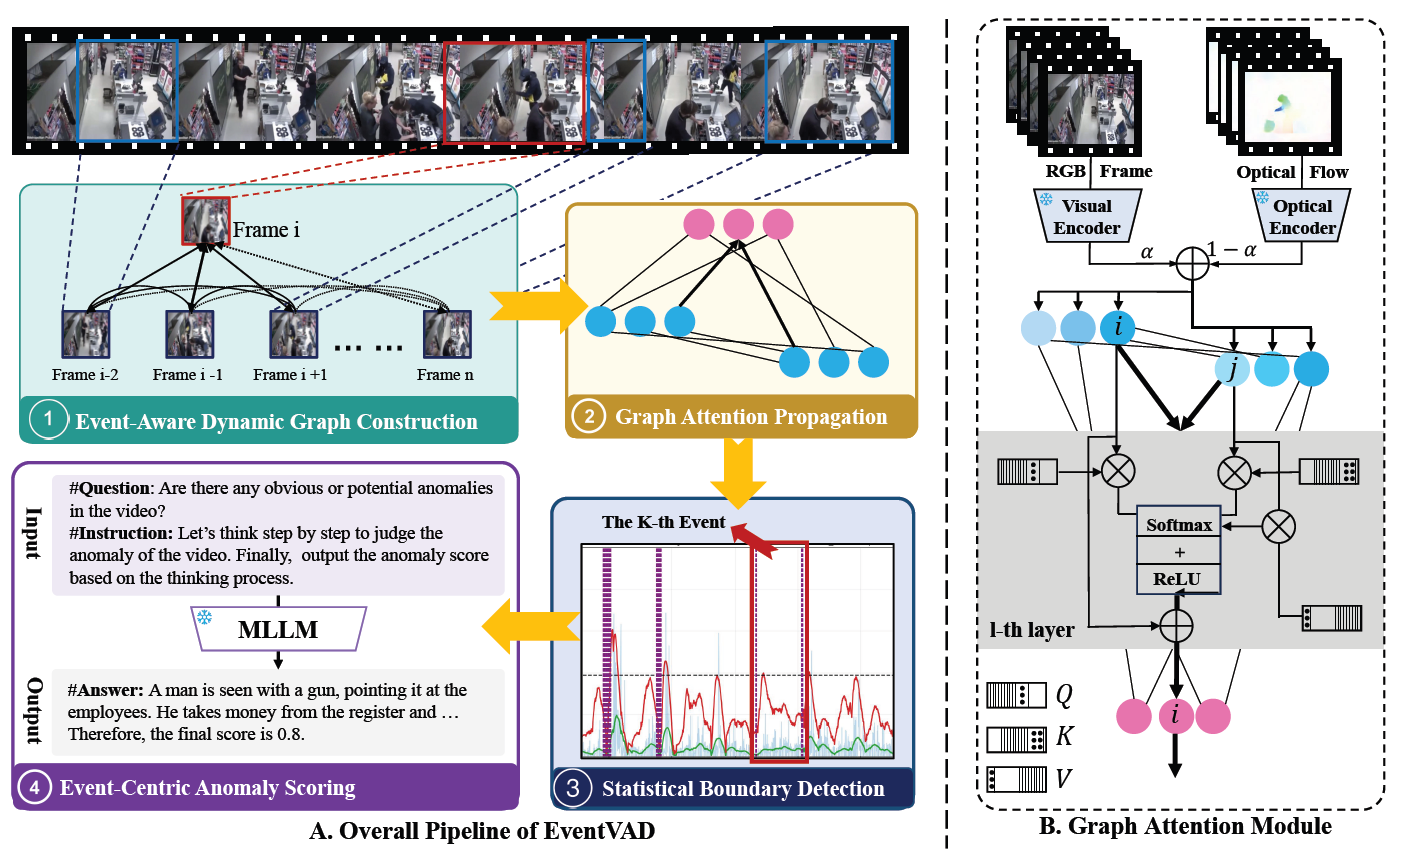
\includegraphics[width=0.6\linewidth]{images/EventVAD_Figure2.png}
			\caption{EventVAD comprises four core modules: (1) Dynamic Graph Construction for establishing spatiotemporal correlations,
				(2) Graph Attention Propagation for refining node features, (3) Statistical Boundary Detection for identifying event transitions
				and boundaries, and (4) Event-Centric Scoring for evaluating anomalies via MLLMs within semantic event units.}
		\end{figure}
		
		\vspace{0.5em}
	\end{frame}
	
	\begin{frame}{Implementation Details}
		\small
		
		\begin{block}{Setting Up}
			We adopt the CLIP ViT-B/16 model to extract $512$-dimensional semantic embeddings, and the pre-trained RAFT model to obtain $128$-dimensional optical flow features, with FPS = 30. We also use bilinear interpolation for spatial alignment to maintain resolution consistency.
		\end{block}
		
		\begin{block}{Backbone and Hyperparameters}
			\begin{itemize}
				\item \textbf{Backbone:} VideoLLaMA2.1-7B-16F
				\item \textbf{Semantic-motion fusion coefficient:} $\alpha = 0.75$
				\item \textbf{Time decay factor:} $\gamma = 0.6$
				\item \textbf{Graph attention propagation iterations:} single iteration
				\item \textbf{Hardware:} single NVIDIA A800 (80GB) GPU
			\end{itemize}
		\end{block}
		
		
	\end{frame}
	
	
	\begin{frame}{Results on UCF-Crime}
		\scriptsize
		
		\begin{table}
			\centering
			\setlength{\tabcolsep}{4pt}
			\renewcommand{\arraystretch}{1.15}
			\begin{tabular}{l l l c c c}
				\hline
				\textbf{Method} & \textbf{Backbone} & \textbf{Supervised} & \textbf{AUC (\%)} \\
				\hline
				RTFM [48] & I3D-RGB & Weakly Supervised & 84.03 \\
				MSL [20] & VideoSwin-RGB & Weakly Supervised & 85.62 \\
				S3R [57] & I3D-RGB & Weakly Supervised & 85.99 \\
				MGFN [4] & VideoSwin-RGB & Weakly Supervised & 86.98 \\
				SSRL [16] & I3D-RGB & Weakly Supervised & 87.43 \\
				CLIP-TSA [14] & ViT & Weakly Supervised & 87.58 \\
				\hline
				BODS [54] & I3D-RGB & One Class & 68.26 \\
				GODS [54] & I3D-RGB & One Class & 70.46 \\
				\hline
				Tur [50] & ResNet & Unsupervised & 65.22 \\
				Tur [51] & ResNet & Unsupervised & 66.85 \\
				DyAnNet [47] & I3D & Unsupervised & 79.76 \\
				\hline
				ZS CLIP [33] & ViT & Training Free & 53.16 \\
				ZS ImageBind (Image) [7] & ViT & Training Free & 53.65 \\
				ZS ImageBind (Video) [7] & ViT & Training Free & 55.78 \\
				LLaVA-1.5 [23] & ViT & Training Free & 72.84 \\
				Video-Llama2 [74] & ViT & Training Free & 74.42 \\
				LAVAD [67] & ViT & Training Free & 78.33 \\
				\textbf{EventVAD} & \textbf{ViT} & \textbf{Training Free} & \textbf{82.03} \\
				\hline
			\end{tabular}
		\end{table}
		
		
	\end{frame}
	
	
	\begin{frame}{Results on XD-Violence}
		\scriptsize
		
		\begin{table}
			\centering
			\setlength{\tabcolsep}{4pt}
			\renewcommand{\arraystretch}{1.12}
			\begin{tabular}{l l l c}
				\hline
				\textbf{Method} & \textbf{Backbone} & \textbf{Supervised} & \textbf{AP (\%)} \\
				\hline
				Wu et al. [59] & I3D-RGB & Weakly Supervised & 73.20 \\
				Wu and Liu [58] & I3D-RGB & Weakly Supervised & 75.90 \\
				RTFM [48] & I3D-RGB & Weakly Supervised & 77.81 \\
				MSL [20] & VideoSwin-RGB & Weakly Supervised & 78.58 \\
				S3R [57] & I3D-RGB & Weakly Supervised & 80.26 \\
				MGFN [4] & VideoSwin-RGB & Weakly Supervised & 80.11 \\
				\hline
				Hasan et al. [9] & AERGB & One Class & 50.32 \\
				Lu et al. [30] & Dictionary & One Class & 53.56 \\
				BODS [54] & I3D-RGB & One Class & 57.32 \\
				GODS [54] & I3D-RGB & One Class & 61.56 \\
				\hline
				RareAnom [46] & I3D-RGB & Unsupervised & 68.33 \\
				\hline
				Blip2 [17] & ViT & Training Free & 10.89 \\
				ZS CLIP [33] & ViT & Training Free & 17.83 \\
				ZS ImageBind (Image) [7] & ViT & Training Free & 27.25 \\
				ZS ImageBind (Video) [7] & ViT & Training Free & 25.36 \\
				LLaVA-1.5 [23] & ViT & Training Free & 50.26 \\
				Video-Llama2 [74] & ViT & Training Free & 53.57 \\
				LAVAD [67] & ViT & Training Free & 60.02 \\
				\textbf{EventVAD} & \textbf{ViT} & \textbf{Training Free} & \textbf{64.04} \\
				\hline
			\end{tabular}
		\end{table}
		
		\vspace{-0.4em}
		\begin{block}{Key Result}
			EventVAD achieves the best training-free performance on XD-Violence as well, confirming strong generalization across datasets.
		\end{block}
		
	\end{frame}
	
	
	\begin{frame}{Ablation Study of Hyperparameters}
		\scriptsize
		
		\begin{table}
			\centering
			\setlength{\tabcolsep}{5pt}
			\renewcommand{\arraystretch}{1.15}
			\begin{tabular}{c c c c c c}
				\hline
				$\gamma \backslash \alpha$ & $0$ & $0.25$ & $0.5$ & $0.75$ & $1$ \\
				\hline
				$0.0$ & 77.92 & 77.13 & 78.47 & 78.91 & 77.34 \\
				$0.2$ & 78.22 & 78.85 & 79.48 & 80.56 & 77.93 \\
				$0.4$ & 78.95 & 79.12 & 79.95 & 81.78 & 79.46 \\
				$0.6$ & 79.89 & 80.67 & 81.57 & \textbf{82.03} & 79.69 \\
				$0.8$ & 78.92 & 79.54 & 80.38 & 81.34 & 79.62 \\
				$1.0$ & 77.12 & 78.81 & 78.75 & 80.97 & 78.97 \\
				\hline
			\end{tabular}
		\end{table}
		
		\vspace{-0.5em}
		\begin{block}{Observation}
			The best performance is achieved at \textbf{$\alpha = 0.75$} and \textbf{$\gamma = 0.6$}, indicating that balanced semantic-motion fusion and moderate temporal decay are crucial for robust anomaly detection.
		\end{block}
		
	\end{frame}
	
\end{document}